\section{Theory}
\label{section:theory}

Following Wentzel \cite{Wentzel27} and later Feshbach \cite{Feshbach58,Feshbach62}
and Fano \cite{Fano61}
the decay width of a decay process initiated by a
primary ionization is given by 

\begin{equation} \label{equation:Fano_golden}
  \Gamma = \sum_\beta 2\pi
           \left| \braket{\Phi|\hat{V}|\chi_{\beta,\varepsilon}} \right|^2 .
\end{equation}

Here, $\ket{\Phi}$ and $\ket{\chi_{\beta,\varepsilon}}$ denote the initial and
final state, respectively. $\hat{V}$ is the interaction operator of the
initial and final states, which in Feshbach's definitions is known as $H_{PQ}$.
The index $\beta$ counts the different
decay channels and $\varepsilon$ denotes the energy of the final state.
Eq. (\ref{equation:Fano_golden}) thereby connects the metastable initial
and the continuum final states. They are constructed by partitioning the
Hamiltonian into two subspaces. The initial (final) state is then an
eigenfunction of this initial (final) state sub-space Hamiltonian.
However, finding proper solutions to both the initial and the final
states on an equal footing is a non-trivial task, because they adhere to
different boundary conditions. Since the final state depends on the energy
of the emitted electron, any approach needs to either determine the continuum
state or to mimic the final state using $\mathcal{L}^2$-functions.
While the continuum functions are normalized with respect to their energy

\begin{equation}
 \braket{\chi_\varepsilon| \chi_{\varepsilon'}} = \delta(\varepsilon-\varepsilon')
\end{equation}

the $\mathcal{L}^2$ approach is based on a discrete set of final states
$\ket{\tilde{\chi}_{\tilde{E}}}$
which adhere to different boundary
conditions and are normalized with respect to space (see e.g. \cite{Craigie14}):
\begin{equation}
 \braket{ \tilde{\chi}_{\tilde{E}_i} | \tilde{\chi}_{\tilde{E}_j} } = \delta_{ij}.
\end{equation}

Because of this different normalization the decay widths are not amenable to
a direct calculation. As first proposed by Hazi \cite{hazi1978}, for
autoionization processes such difficulties
can be solved by using the
Stieltjes-Chebyshev moment theory also called Stieltjes imaging
\cite{Langhoff76,Corcoran77,MuellerPlathe90}.
It relies on the observation that the moments of the projected final
state Hamiltonian $H_f$

\begin{equation}
 \mu_k = \braket{ \Phi | \hat{V} H^k_f \hat{V} | \Phi }
\end{equation}

calculated from the determined
discrete pseudo-spectrum are good approximations to the moments determined
from the real continuum states.
This can be shown by inserting the resolution of identity for
the continuum states

\begin{equation}
 \mu_k = \sum_i \varepsilon_i^k
         \left| \braket{ \Phi | \hat{V} | \chi_{i,\varepsilon} } \right| ^2
       + \int\limits_{E_{thr}}^{\infty} \varepsilon^k
         \left| \braket{\Phi|\hat{V}|\chi_{\varepsilon}} \right|^2 \mathrm{d}\varepsilon  .
\end{equation}

Since the non-zero contribution to the coupling matrix elements in the
Feshbach-Fano approach stem only
from an interaction region of finite size, where the $\mathcal{L}^2$ final
state functions are nonvanishing, we may replace the expansion
$\sum\limits_i \ket{\chi_{i,\varepsilon}} \bra{\chi_{i,\varepsilon}}
 + \int \mathrm{d}\varepsilon \ket{\chi_\varepsilon} \bra{\chi_\varepsilon}$
by its $\mathcal{L}^2$ approximation
$\sum\limits_j \ket{\tilde{\chi}_{\tilde{E}_j}} \bra{\tilde{\chi}_{\tilde{E}_j}}$
(see \cite{Reinhardt79})

\begin{equation}
 \label{eq:moment_discrete}
 \mu_k \approx \sum\limits_j \tilde{E}_j ^k
         \left| \braket{\Phi|\hat{V}|\tilde{\chi}_{\tilde{E}_j}}  \right|^2 .
\end{equation}

Then the decay width can be determined through a series of
consecutive approximations to the moments of increasing order $k$.

To achieve this kind of description, we choose the non-relativistic
FanoADC-Stieltjes approach, described
in the next sections. Here, the ADC is used for the description of the
initial and final states and the resulting discrete pseudo-spectrum
is then subject to a Stieltjes imaging procedure.
An exhaustive description of the method can be found in \cite{Fasshauer_thesis}.

\subsection{ADC}

\label{section:adc}

The {ADC} is a Green's function approach, which is a method for the
calculation of ionization
energies and electron affinities.
Its advantage is the ability to determine the desired ionization energies
without explicit calculation of the initial and final states, but instead
obtaining their energy differences directly.
Moreover, this approach is size-consistent and is hence
suitable for the description of larger systems. \cite{Mertins96_1}

Originally, the Green's function was formulated in the Dyson ansatz and
determined using perturbation theory \cite{Schirmer82_1,Schirmer83}.
This way both the ionization and the
electron affinity part had to be included in the description. In the non-Dyson
scheme those two are separable and hence, the dimension of the problem is reduced
when one is interested in either the $N+1$ (electron affinity)
or the $N-1$ (ionization energy) part \cite{Schirmer98}

\begin{equation} \label{adc_ion_attach}
 G_{pq}(\omega) = G^+_{pq}(\omega) + G^-_{pq}(\omega) .
\end{equation}

The ionization part $ G^-_{pq}(\omega)$
is a function of the ionization energies
$\omega$ and is transposed to give
$\tilde{G}^-_{pq}(\omega) = G^-_{qp}(\omega)$.
It can be cast to the compact and orthogonal form

\begin{equation}\label{matrixspec}
\mathbf{\tilde{G}}^-(\omega) = \mathbf{x}^\dagger
                               (\omega\mathds{1}-\mathbf{\Omega})^{-1}\mathbf{x} 
\end{equation}

where $\mathbf{x}$ are the spectroscopic amplitudes and $\mathbf{\Omega}$ is
the diagonal matrix of energy eigenvalues.
This diagonal representation can be reformulated using so-called
\emph{intermediate states} (IS) \cite{Schirmer91}.
%These are formally constructed from Correlated Excited States (CES),
%which are constructed
%using the same kind of excitation operators as in an {CI} expansion.
%In contrast to the {CI} approach, the {CES}
%are constructed from these operators
%acting on the exact and therefore correlated groundstate rather than the
%Hartree Fock ground state. These {CES} are then
%grouped into excitation classes
%and these classes are orthogonalized with respect to each other. Afterwards,  
%the states within each class are orthogonalized \cite{Mertins96_1}.

\begin{equation}\label{isradc}
\mathbf{\tilde{G}}^-(\omega) = \mathbf{f}^\dagger(\omega\mathds{1}-\mathbf{M})^{-1}\mathbf{f}
\end{equation}

Here $\mathbf{M}$ denotes the {ADC} matrix and $\mathbf{f}$ denotes
the effective transition moments.

By inspection of both Eq. (\ref{matrixspec}) and (\ref{isradc}),
the ionization energies
are poles of $\mathbf{\tilde{G}}^-(\omega)$, which can be determined by
solving the eigenvalue problem
\begin{equation}\label{adcewp}
\mathbf{M} \mathbf{Y} = \mathbf{Y}\mathbf{\Omega} \quad\text{with } \mathbf{Y}^\dagger\mathbf{Y}=\mathbf{1}
\end{equation}

The spectroscopic amplitudes $\mathbf{x}$ can then be obtained from the
effective transition moments $\mathbf{f}$ as

\begin{equation}
 \mathbf{x} = \mathbf{Y}^\dagger \mathbf{f}
\end{equation}

To this point, the approach is exact.
For the actual construction of the {ADC} matrix $\mathbf{M}$ and the
effective transitions moments $\mathbf{f}$, both
are expanded into orders of perturbations based on the
M{\o}ller-Plesset partitioned Hamiltonian.

\begin{eqnarray}
\mathbf{M} &=& \mathbf{M}^{(0)} + \mathbf{M}^{(1)} + \mathbf{M}^{(2)} + \cdots\label{stf}\\
\mathbf{f} &=& \mathbf{f}^{(0)} + \mathbf{f}^{(1)} + \mathbf{f}^{(2)} + \cdots\label{stf}
\end{eqnarray}

From these, different orders of perturbation theory of the Hamiltonian can be
constructed successively in terms of correlated $N-1$ particle states ($1h$,
$2h1p$, \dots).
Hereby, the truncation after the $n$-th order leads
to ADC($n$). The contributions to the different classes for different
orders of {ADC} are shown
in Figure \ref{figure:adcmat_pgf} \cite{Trofimov05}.

\begin{figure}[h]
  \centering
  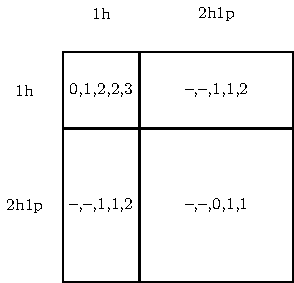
\includegraphics{pics/adcmat_pgf.pdf}
  %\input{pics/adcmat_pgf}
  \caption{Schematic illustration of an {ADC}($n$) matrix for different orders
           of perturbation for $n=0,1,2,2x,3$. In the illustration, the respective
           highest order contribution is shown for the different blocks.
           Hence, ADC(2x) is an extended ADC(2) including first
           order contributions to the satellite block.}
  \label{figure:adcmat_pgf}
\end{figure}

The matrix elements of ADC(2x) are explicitly given by
\begin{itemize}
 \item $1h/1h$ ($1h$ block):
   \begin{align}
    M_{kk'}^{(0)} &= \varepsilon_k \delta_{kk'} \\
    M_{kk'}^{(1)} &= 0 \\
    M_{kk'}^{(2)} &= -\frac12 \sum\limits_{abl} V_{ab[kl]} V_{k'l[ab]} %\times
                     \frac{\varepsilon_a+\varepsilon_b-\varepsilon_l
                       -\frac12 \varepsilon_k-\frac12 \varepsilon_{k'}}
                     {(\varepsilon_a+\varepsilon_b-\varepsilon_k-\varepsilon_l)
                      (\varepsilon_a+\varepsilon_b-\varepsilon_{k'}-\varepsilon_l)}
   \end{align}
 \item $1h/2h1p$ (coupling block):
   \begin{equation}
    M_{j,akl}^{(1)} = V_{kl[aj]}
   \end{equation}
 \item $2h1p/2h1p$ (satellite block):
   \begin{align}
    M_{akl,a'k'l'}^{(0)} &= (-\varepsilon_a+\varepsilon_k+\varepsilon_l)
                             \, \delta_{aa'}\delta_{kk'}\delta_{ll'} \\
    M_{akl,a'k'l'}^{(1)} &= -\delta_{aa'} V_{k'l'[kl]} + \delta_{kk'} V_{al'[a'l]}
                            +\delta_{ll'} V_{ak'[a'k]} - (k \leftrightarrow l)
   \end{align}
\end{itemize}

Here, $\varepsilon_r$ denotes the $r$-th Hartree Fock orbital energy.
The occupied states are labelled
by $i,j,k,\dots$ and the unoccupied states are labelled by $a,b,c,\dots$. The
two-electron integrals for any combination of occupied and unoccupied orbitals
labelled by $p,q,r,s$ read as
\begin{equation}
 V_{pqrs} = \braket{\varphi_p(1)\varphi_q(2) |V(1,2)| \varphi_r(1)\varphi_s(2)}
\end{equation}

and $V_{pq[rs]} = V_{pqrs} - V_{pqsr}$.


These equations can also be used in the relativistic case based on
Dirac-Hartree-Fock orbital energies as well as integrals
\cite{Pernpointner04_1,Pernpointner04_2}  and using the
no-pair approximation (see e.g. \cite{ReiherWolf09}). This
approximation ensures that pair creation processes are excluded from
the calculation by allowing annihilation and creation operators
$c_p$ and $c_q^\dagger$ in the
spectral representation
\begin{equation}
 G^-_{pq}(\omega) = \sum\limits_{n\in \{N-1 \}}
                    \frac{\braket{\Psi_0^N| c_q^\dagger | \Psi_n^{N-1}}
                          \braket{\Psi_n^{N-1}| c_p |\Psi_0^{N-1}}}
                    {\omega + E_n^{N-1} - E_0^N -i\eta}
\end{equation}

of Eq. (\ref{adc_ion_attach})
to operate on the space of positive energy solutions only. Since energies
high enough to overcome the gap of $2mc^2$ are hardly achieved in chemistry,
this approximation is reasonable.




\subsection{FanoADC}
In the FanoADC, the discrete ADC Hamiltonian
is used for the construction of the pseudo-spectrum of the total decay width
$\Gamma$.
Due to multiple possible final states, the procedure
of Feshbach \cite{Feshbach62}
using projection operators for the partitioning of the Hamiltonian
into an initial and a final state subspace is employed.
The processes of interest start from a singly ionized initial state and end in
a doubly ionized final state with an addi\-tio\-nal electron
in the continuum.
Therefore, the basis functions for the description of the entire final
state subspace are chosen from
the $2h1p$ class of configurations, where the $2h$ part is assumed to
describe the doubly ionized final state and the
particle represents the electron in the continuum. This approach can be justified
by rewriting the spectral moments (see Eq. (\ref{eq:moment_discrete}))
of the decay width $\Gamma$
(Eq. (\ref{equation:Fano_golden})) explicitly:

\begin{align}
  \tilde{\Gamma}_k &= 2\pi \mu_k \\
         &= 2\pi \sum_j \tilde{E}_j^k
            \braket{\Phi|\hat{V}|\tilde{\chi}_{\tilde{E}_j}}
            \braket{\tilde{\chi}_{\tilde{E}_j}|\hat{V}|\Phi} \\           
         &\approx 2\pi \sum_q \left( E^{2h1p}_q\right) ^k
            \braket{\Phi|\hat{V}|\chi^{2h1p}_q}
            \braket{\chi^{2h1p}_q|\hat{V}|\Phi}
\end{align}

%where the complete set of ADC eigenstates in the final state subspace
%$\ket{\tilde{\chi}_{\tilde{E}_j}}$ is used for the $\mathcal{L}^2$ representation
%of the decay continuum.
One may interpret the set of final states as a complete basis
of the final state subspace.
This might be replaced by any other complete basis
describing the outgoing electron. The idea of the FanoADC is to choose
the manifold of $2h1p$ states describing the decay to replace this
complete basis.
As shown in \cite{Averbukh05}, this basis is not required to yield the
exact energies of the different channels as long as it spans the space
of interest.
The manifold of $2h1p$ states is formally not complete, but
yields a proper description when the ionization of the system can be
described reasonably well in the single-particle picture.
Additionally, one has to consider the error introduced
by using an incomplete basis set on the Hartree-Fock level and the truncation
of the virtual space in the post Hartree-Fock procedure.

Not all $2h1p$ states describe energetically allowed final states.
The energy conservation $E_{in} = E_{A^{2+}} + E_{e^-_{sec}}$ has
to be satisfied, which is only possible for $E_{A^{2+}} < E_{in}$, where
$E_{in}$ denotes the initial state energy, $E_{A^{2+}}$ the energy of the
doubly ionized part of the final state and $E_{e^-_{sec}}$ denotes the
kinetic energy of the secondary electron emitted in the process.
If the energy of
the doubly charged system is higher than the energy of the initial state, the
process is energetically forbidden. Hence, all $2h1p$ states characterized by
a $2h$ contribution with an energy higher than the initial state energy will
not contribute to the final states.
Instead, these $2h1p$ states can be used to improve the description of
the initial state.
The partitioning into initial and final state configurations can be
achieved based on Hartree-Fock orbital occupations by manual choice of $2h$
configurations
or in an energy-based approach as described by Averbukh
\cite{Averbukh05}.
In this work, we employ the partitioning by population and manually include
those configurations which correspond to open channels.
% regardless its
%inability to distinguish one- and two-site ionized final states in
%non-spherical systems with inversion symmetry.

\begin{figure}[h]
  \centering
  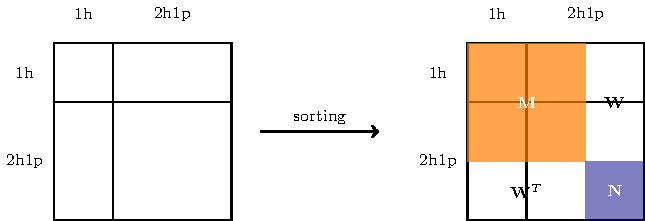
\includegraphics[scale=0.7]{pics/fano_matsort_pgf.pdf}
  \caption{Schematic illustration of the partitioning of the ADC matrix
           according to the projection operators of the initial and final
           states.}
  \label{figure:fano_matsort}
\end{figure}

The partitioning is therefore achieved as follows:
All $2h1p$ configurations characterized by a $2h$
part corresponding to one of the
final state configurations of possible decay channels
are chosen to be part of the final state subspace.
All $1h$ configurations and those $2h1p$ configurations not corresponding
to a possible final state configuration are used for the description
of the initial state. This leads to a resorted ADC matrix as shown in
Figure \ref{figure:fano_matsort}, where the subspace of the initial state
is denoted by $\mathbf{M}$, the final state subspace by $\mathbf{N}$, and
the interaction coupling those two subsets is named $\mathbf{W}$.
Speaking in terms of Feshbach's projection operators, where $\mathbf{P}$
denotes the projector for the final state subspace acting on the full
Hamiltonian of the system $\mathbf{H}$ and
$\mathbf{Q}=\mathds{1}- \mathbf{P}$
denotes the projector for the initial state subspace, these subspaces are
given by $\mathbf{M}=\mathbf{Q}\mathbf{H}\mathbf{Q}$ and
$\mathbf{N} = \mathbf{P}\mathbf{H}\mathbf{P}$.


The separate diagonalization of the initial and final state subspaces
$\mathbf{M}$ and $\mathbf{N}$ yields
the corresponding eigenvectors and eigenvalues on the diagonal of the
matrices $\mathbf{\Lambda}$ and $\mathbf{\Omega}$

\begin{align}
  \mathbf{\Lambda} &= \mathbf{I}^T \mathbf{M} \mathbf{I}  \\
  \mathbf{\Omega}  &= \mathbf{F}^T \mathbf{N} \mathbf{F} 
\end{align}

and the Hamiltonian is represented in the basis of their eigenstates
as illustrated in
Figure \ref{figure:fano_bastrans} with $\mathbf{V} = \mathbf{I}^T \mathbf{W} \mathbf{F}$
being the interaction part
in this new basis. It has to be noticed that $\mathbf{\Omega}$ in this
definition is the matrix of final state subspace eigenvalues and
does not equal the eigenvalue matrix of the full ADC matrix in Eq.
(\ref{matrixspec}).

\begin{figure}[h]
  \centering
  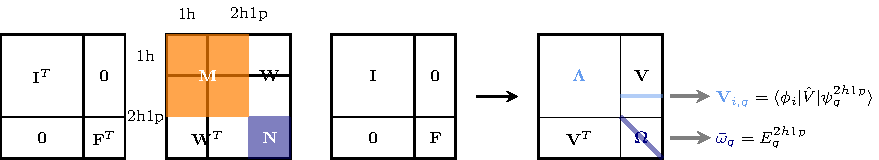
\includegraphics[scale=1.0]{pics/fano_bastrans_pgf.pdf}
  \caption{Schematic illustration of the basis transformation of the full ADC
           matrix into the basis of initial and final states. The pseudo-spectrum
           is given by the manifold of $\bar{\omega}_q$ and
           $V_{i,q} = \braket{\phi_i |\hat{V}| \psi_{q}^{2h1p}}$.}
  \label{figure:fano_bastrans}                                        
\end{figure}

In general, neither of the final state energies $\bar{\omega}_q$
equals the resonance energy. Therefore, the pseudo-spectrum enters
the Stieltjes calculation.
For a specific choice of the initial state $i$
this pseudo-spectrum is given by the
manifold of final state energies                                      
$\bar{\omega}_q$ and the corresponding interaction part in the        
basis of the initial and                                              
final subspace eigenstates                                                     
$V_{i,q} = \braket{\phi_i |\hat{V}| \psi_{q}^{2h1p}}$.




\subsection{Stieltjes Imaging}
In general, Gaussian quadrature is a numerical method to solve integrals.
From the discrete pseudo-spectrum consisting of $\bar{\omega}_q$
and $V_{i,q} = \braket{\phi_i |\hat{V}| \psi_{q}^{2h1p}}$,
$N$ pairs of optimal abscissae ($1/\omega_i$)
and weights $f_i$ for a Gaussian quadrature can be obtained using
Chebyshev polynomials as elaborately described in \cite{MuellerPlathe90}.
These are then used for the construction of inverse moments, which
are preferred to normal moments because of their convergence behaviour

\begin{equation}
  S(-k) = \int\limits_{E_{thr}}^{\infty} \omega^{-k} \, \mathrm{d}F(\omega)
       = \int\limits_{E_{thr}}^{\infty} \omega^{-k} f(\omega) \, \mathrm{d}\omega
       \approx \sum\limits_{i=1}^N \left(\frac{1}{{\omega}_i}\right)^k f_i .
\end{equation}

The inverse moments are in terms of Gaussian quadrature
connected to both the distribution function
$F(\omega)$ and a density function $f(\omega)$. In the particular case of
interest, the density function $f(\omega)$ equals the decay width $\Gamma(E)$
(see Eq. (\ref{eq:moment_discrete})).
The procedure and the background shortly
explained here can be found in detail in \cite{Reinhardt79,
MuellerPlathe89,Corcoran77,Langhoff76}. For convenience, we from this point
on write the optimal abscissae $\frac{1}{\omega_i}$ as $\varepsilon$.

Having obtained the optimal abscissae and weights, the probability
distribution function
$F(\varepsilon)$ can be approximated. For this purpose, the so-called Stieltjes imaging
is employed, where

\begin{equation}
  F^{(n)} (\varepsilon) =
  \begin{cases}
    0                                & \varepsilon   < \varepsilon_1\\
    \sum\limits_{j=1}^{i} f_j        & \varepsilon_i < \varepsilon < \varepsilon_{i+1}\\
    \sum\limits_{j=1}^{n} f_j = S(0) & \varepsilon_n < \varepsilon .
  \end{cases}
\end{equation}
                                                                  
This procedure is based on the so-called Chebyshev inequalities
                                                                  
\begin{equation} \label{equation:Chebyshev_inequalities}          
  F^{(n)}(\varepsilon_i - 0) \le F^{(n+1)}(\varepsilon_i - 0) \le F(\varepsilon_i)
  \le F^{(n+1)}(\varepsilon_i + 0) \le F^{(n)}(\varepsilon_i + 0).          
\end{equation}                                                    
                                                                  
This means that the distribution functions obtained from the Chebyshev
polynomials approaching the abscissae $\varepsilon_i$ from below
and from above      
give lower and upper bounds to the actual value of the distribution
function at this particular point $F(\varepsilon_i)$. In fact, the mean of these     
two values usually is a very good approximation to the exact value:

\begin{equation}                                                  
  F^{(n)} (\varepsilon_i) = \frac 12 \left[ F^{(n)} (\varepsilon_i - 0)     
                       + F^{(n)} (\varepsilon_i+0) \right]             
\end{equation}                                                    
                                                                  
Since the integral was evaluated and not the density function as such
the distribution function obtained from the
discrete pseudo-spectrum is normalized correctly (see \cite{Reinhardt79}).
This distribution function is then numerically differentiated via 
                                                                  
\begin{equation}                                                  
  f^{(n)} (\varepsilon) =                                              
  \begin{cases}                                                   
    \frac 12 \frac{f_1}{\varepsilon_1}    & \varepsilon < \varepsilon_1\\        
    \frac 12 \frac{f_{i+1} + f_i}{\varepsilon_{i+1} - \varepsilon_i}        
                                   & \varepsilon_i < \varepsilon < \varepsilon_{i+1}\\
    0                              & \varepsilon_n < \varepsilon
  \end{cases}                                                     
\end{equation}                                                    
                                                                  
to give  $r-1$ non-zero points of the desired                     
density function $f(\varepsilon)$, which are                           
subsequently interpolated.
In the routine of Averbukh, a          
monotonicity-preserving piecewise cubic Hermite spline interpolation
is used for this purpose. Afterwards, the interpolated density function is evaluated
for the energy of interest, which is the resonance energy $E_r$ in case of the  
autoionization processes to give the decay width $\Gamma$. 
Finally, convergence of the decay widths with increasing orders of
moments is investigated.

Unfortunately the procedure to obtain the optimal abscissae and weights
involves the subtraction of two large numbers, which
leads to numerical instabilities in high order moments. Therefore, they have to
be checked carefully and only trustworthy moments should be
used for the evaluation of the decay widths.
This can be achieved by inspection of abscissae and weights of each order.
Since the decay width $\Gamma(E)$ is a smooth function
unphysical oscillations in the curve constructed
from the abscissae and weights of one order of moments indicate numerical
instabilities in this particular order.
If this behaviour is observed, the abscissae and weights obtained from this
order of moments and all higher orders are discarded.
Finally, the abscissae
and weights from the remaining, consecutive orders of moments enter
the interpolation scheme.
